\documentclass[12pt]{article}
\usepackage[margin=1in]{geometry}
\usepackage{amsmath,amssymb,amsthm,booktabs,graphicx,natbib,microtype,array}
\newtheorem{theorem}{Theorem}
\newtheorem{proposition}[theorem]{Proposition}
\newtheorem{corollary}[theorem]{Corollary}
\newtheorem{remark}[theorem]{Remark}
\newcommand{\K}{\mathcal K}
\title{Temporal Anchors and the Recursive Packet-Transport Wall\\\large A Typed Source Repair and Outward Radius Audit}
\author{Prime Dynamics Theory Program}
\date{July 2026}

\begin{document}
\maketitle

\begin{abstract}
RH-149 proposed propagating the ten RH-142 spectral-packet balls through the
RH-143 threshold branches of the RH-96 recursive refresh.  We show first that
this composition is not type-correct.  RH-142 certifies a rank-four packet of
the postblock state $A^{H(\sigma)}S$, whereas RH-96 starts at time zero from
the source $S$ and uses clock ranks $4,5,6,6,7$.  Orthogonal projectors of
different ranks have operator distance one.  Eight channels therefore fail
by rank alone; on the two rank-four channels, the temporal center distances
are $0.8652$ and $0.9963$, and adding the inherited radii $0.6097$ and
$0.9574$ makes both transferred balls vacuous.  None of the ten RH-142 balls
is an informative RH-96 seed.

We repair both types.  At time zero we use the native clock rank and enclose
the exact-binary moving-memory Grams around their numerical centers in
384-bit Arb arithmetic.  All ten source packets certify; the smallest source
gap is $3.303\times10^{-4}$ and the largest projector radius is
$2.876\times10^{-13}$.  We then prove an outward one-step recursion through
the projected cross, clipped threshold branch, selected left-singular
subspace, enriched projector, and Ritz packet.  The direction gate correctly
uses $s_4-s_5$ when the clock rank exceeds four, even though maximum clipping
makes $s_5$ irrelevant to the branch count.

The repaired finite audit still closes no complete chain.  Seventeen updates
certify in total, but every channel stops at update two or three: seven first
at the branch gate and three first at the Ritz gate.  The smallest decisive
failure ratio is $1.506$.  This is a universal-information obstruction, not a
disproof of the exact recursion.  It redirects the next layer toward a joint,
gauge-free output-packet enclosure that avoids separately resolving weak
enrichment directions.
\end{abstract}

\section{Packet balls carry time and rank types}
Let $P_{t,r}$ denote a rank-$r$ orthogonal packet projector attached to time
$t$.  A ball around $P_{t,r}$ is not an untyped approximation to every packet
appearing elsewhere in a construction.  Both labels matter before any
perturbation theorem can be composed.

\begin{theorem}[Typed anchor compatibility]\label{thm:typed}
Let $P,Q$ be finite-dimensional orthogonal projectors.
\begin{enumerate}
\item If $\operatorname{rank}P\ne\operatorname{rank}Q$, then
      $\|P-Q\|=1$.
\item If the ranks agree and $\|\widetilde P-P\|\leq\rho$, then
\[
 \|\widetilde P-Q\|\leq
 \min\{1,\|P-Q\|+\rho\}.
\]
Consequently an inherited radius is informative at the target anchor only
when the ranks agree and the transferred upper is below one.
\end{enumerate}
\end{theorem}
\begin{proof}
If $\operatorname{rank}P>\operatorname{rank}Q$, dimension counting gives a
unit vector $v\in\operatorname{ran}P\cap\ker Q$.  Hence
$(P-Q)v=v$, while the difference of two orthogonal projectors has norm at
most one.  Interchanging $P,Q$ handles the other rank ordering.  The second
claim is the triangle inequality together with the unit diameter of the
projector metric.
\end{proof}

The theorem immediately exposes the proposed interface error.  RH-142 uses
rank four at time $H(\sigma)$.  RH-96 uses ranks $4,5,6,6,7$ at time zero.
Thus eight transfers are exactly unit radius.  For $\sigma=0.16$, where the
ranks agree, the two center-distance-plus-radius sums are $1.4749$ and
$1.9537$.  Capping at one again leaves no information.

Merely moving the RH-142 rank-four truncation to time zero is also not a
uniform repair.  If $p_i$ are normalized squared source singular values,
$q=\sum_{i>4}p_i$, and $c=1-q$, the exact ideal-truncation formulas are
\[
 g_4=\frac{p_4}{c},\qquad
 e_4=\max\!\left\{p_5,\frac{q p_1}{c}\right\}.
\]
Only three of ten frozen source spectra satisfy $g_4>2e_4$.  This diagnostic
assumes an ideal SVD and is not itself an interval certificate, but it shows
why the native clock rank must be retained.

\section{Source-aligned repair}
Write
\[
 G_0=\frac{S^*S}{\|S\|_F^2},\qquad
 G_t=\frac{S_t^*S_t}{\|S_t\|_F^2}+\eta G_{t-1},
 \quad S_t=A^tS,\quad \eta=2^{-9}.
\]
The exact model treats every archived fp64 entry of $A,S$ as its exact binary
value.  At each time the audit evaluates the normalized snapshot and memory
recurrence in 384-bit Arb arithmetic, then encloses it around the archived
fp64 Gram $B_t$.  We use the Frobenius upper as an operator radius
$\delta_t$.

For the source center $B_0$, a symmetric eigendecomposition supplies the
clock-rank gap; its reconstruction error and a conservative local backward
proxy are subtracted twice.  If the resulting gap $g_0$ obeys
$g_0>2\delta_0$, Davis--Kahan gives \citep{DavisKahan1970,Bhatia2007}
\[
 \epsilon_0\leq\frac{\delta_0}{g_0-\delta_0}.
\]
All ten source packets pass.  The minimum $g_0$ is
$3.303289\times10^{-4}$, the maximum memory-Gram radius over every audited
time is $2.642\times10^{-15}$, and
$\max\epsilon_0=2.876\times10^{-13}$.  The corrected seed is therefore
extremely tight; the subsequent loss does not originate at the source.

\section{Outward recursive transport}
For a Hermitian Gram $B$ and rank-$r$ packet $Q$, define the projected cross
\[
 \K(B,Q)=(I-Q)BQ.
\]
Suppose exact objects $\widetilde B,\widetilde Q$ satisfy
\[
 \|\widetilde B-B\|\leq\delta,qquad
 \|\widetilde Q-Q\|\leq\epsilon,qquad \|B\|\leq b.
\]
The first outward radius is
\begin{equation}\label{eq:cross}
 \eta_K=\delta+2b\epsilon,qquad
 \|\K(\widetilde B,\widetilde Q)-\K(B,Q)\|\leq\eta_K.
\end{equation}
Indeed, split the matrix perturbation from the projector perturbation and
use
\[
 \K(B,P)-\K(B,Q)=(Q-P)BP+(I-Q)B(P-Q).
\]

Let $s_1\geq s_2\geq\cdots$ be the nominal cross singular values.  The RH-96
policy clips the relative threshold $\tau=10^{-8}$ to widths
$2\leq w\leq4$.  RH-143 gives the exact open branch radius
\[
 \beta=\min\left\{
 \frac{s_w-\tau s_1}{1+\tau}\ (w>2),\quad
 \frac{\tau s_1-s_{w+1}}{1+\tau}\ (w<4)
 \right\},
\]
where irrelevant clipped sides are omitted.  The branch is fixed when
$\eta_K<\beta$.

Branch stability does not identify the selected direction space.  Put
\[
 \gamma=s_w-s_{w+1},
\]
using the actual next singular value.  In particular, when $w=4$ and
$r>4$, one must use $s_5$ rather than zero.  Wedin's theorem gives, under
$\gamma>2\eta_K$ \citep{Wedin1972,StewartSun1990},
\begin{equation}\label{eq:direction}
 \|\widetilde D-D\|\leq
 \epsilon_D:=\frac{\eta_K}{\gamma-\eta_K}.
\end{equation}
Here $D,\widetilde D$ are the selected left-singular projectors.  Since each
direction space is orthogonal to its input packet, the enriched projectors
$E=Q+D$ obey
\[
 \|\widetilde E-E\|\leq
 \epsilon_E:=\min\{1,\epsilon+\epsilon_D\}.
\]

Finally set $H=EBE$ and $\widetilde H=\widetilde E\widetilde B\widetilde E$.
Then
\begin{equation}\label{eq:ritz}
 \|\widetilde H-H\|\leq
 \zeta:=\delta+2b\epsilon_E.
\end{equation}
If the nominal rank-$r$ Ritz gap $g_R$ satisfies $g_R>2\zeta$, the output
packet radius is
\[
 \epsilon^+=\frac{\zeta}{g_R-\zeta}.
\]

\begin{theorem}[One-step packet transport]\label{thm:transport}
If the branch, direction, and Ritz inequalities above are all strict, then
the exact update takes the same clipped width as the nominal update and its
rank-$r$ output projector lies in the radius-$\epsilon^+$ ball around the
nominal Ritz packet.
\end{theorem}
\begin{proof}
Equation~\eqref{eq:cross} and singular-value Weyl bounds place every exact
cross singular value in its nominal $\eta_K$ interval.  The sharp RH-143
branch radius fixes the clipped count.  Wedin's theorem gives
\eqref{eq:direction}; orthogonality gives the enriched-projector sum; and
expanding $\widetilde E\widetilde B\widetilde E-EBE$ gives
\eqref{eq:ritz}.  Davis--Kahan at the Ritz gap completes the update.
\end{proof}

The strict gates are universal-information barriers.  At a threshold
contact the clipped branch can change.  If a singular or Hermitian gap is at
most twice its perturbation radius, diagonal two-mode examples permit the
selected and omitted values to meet or reverse.  A particular correlated
exact matrix may still behave well, but norm-ball data alone cannot identify
which side occurs.

\section{Finite obstruction audit}
The audit applies Theorem~\ref{thm:transport} sequentially and stops at the
first failed gate; it never substitutes a nominal branch after certification
is lost.  Local fp64 cross and Ritz backward proxies are charged in addition
to the Arb Gram radii.  Table~\ref{tab:audit} records the result.  ``Ratio''
means $\eta_K/\beta$ at a branch wall or $2\zeta/g_R$ at a Ritz wall, so a
failure has ratio at least one.

\begin{table}[t]
\centering
\scriptsize
\begin{tabular}{cccrccc}
\toprule
$\sigma$ & side & rank & source radius & certified updates & first wall & ratio\\
\midrule
0.16 & L & 4 & $5.36\!\times\!10^{-15}$ & 1 & branch & $1.52\!\times\!10^8$\\
0.16 & R & 4 & $2.65\!\times\!10^{-15}$ & 1 & branch & $3.94\!\times\!10^8$\\
0.08 & L & 5 & $3.77\!\times\!10^{-15}$ & 1 & Ritz & $1.23\!\times\!10^2$\\
0.08 & R & 5 & $6.88\!\times\!10^{-15}$ & 2 & branch & $4.62\!\times\!10^6$\\
0.04 & L & 6 & $2.90\!\times\!10^{-14}$ & 2 & branch & $48.4$\\
0.04 & R & 6 & $5.30\!\times\!10^{-15}$ & 2 & branch & $2.98$\\
0.02 & L & 6 & $9.66\!\times\!10^{-14}$ & 2 & branch & $1.51$\\
0.02 & R & 6 & $1.29\!\times\!10^{-14}$ & 2 & Ritz & $32.9$\\
0.01 & L & 7 & $2.88\!\times\!10^{-13}$ & 2 & branch & $5.11$\\
0.01 & R & 7 & $4.66\!\times\!10^{-14}$ & 2 & Ritz & $4.27$\\
\bottomrule
\end{tabular}
\caption{Source-aligned outward transport at the primary threshold.}
\label{tab:audit}
\end{table}

There are 17 certified recursive updates, but no complete chain.  Seven
channels first fail the branch gate; all seven simultaneously fail the
rank-aware direction gate.  Three first fail only after enrichment, at the
Ritz gap.  The nearest decisive wall is the $\sigma=0.02$ left branch with
ratio $1.5056$; the others range to $3.94\times10^8$.

\begin{figure}[t]
\centering
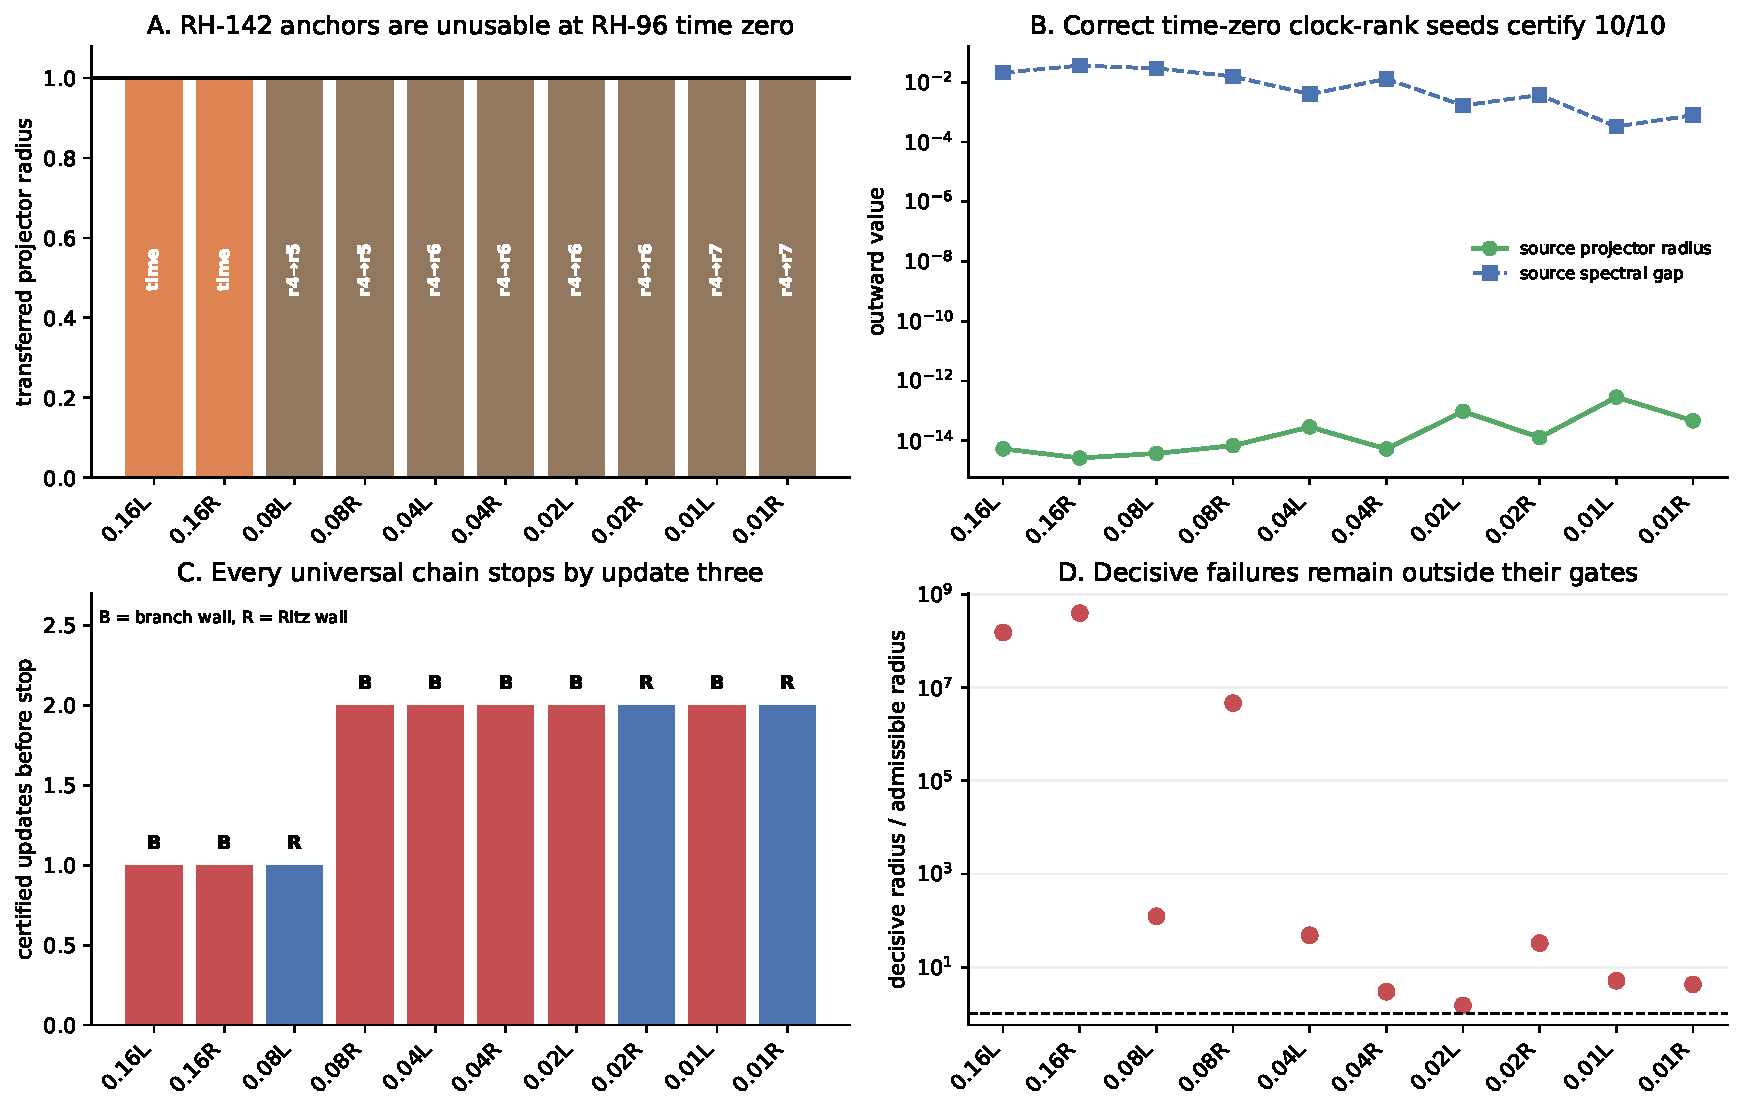
\includegraphics[width=\textwidth]{figures/temporal_anchor_packet_transport.pdf}
\caption{Inherited type obstruction, corrected source packets, certified
prefix lengths, and decisive failure ratios.}
\label{fig:audit}
\end{figure}

The broad radii are generated after one or two updates even though the source
radii are tiny.  The separated construction first resolves a weak direction
subspace and only then asks whether its enriched Ritz packet is stable.  When
$s_4-s_5$ is small, direction uncertainty is amplified before the Ritz step;
the next cross can then exceed even a positive nominal branch margin.

\section{Route consequence and claim boundary}
The original RH-149 instruction ``propagate the RH-142 packet balls through
RH-143'' cannot be executed: those balls have the wrong temporal or rank
type.  Correcting the seed removes that problem completely but exposes the
next one.  The modular norm-ball route loses correlation between the input
packet, cross, selected weak directions, and output Ritz packet.

The next layer should therefore enclose the output packet jointly, for
example through a graph transform, block Riccati equation, residual theorem,
or contour projector.  Such a result may bypass unstable coordinates inside
a weak direction cluster.  A fallback is to define a new recursion whose
native start is the postblock horizon certified by RH-142.  Transported
outward assembly must wait until one of these routes closes a complete packet
chain.

We have proved a typed-anchor theorem, a one-step outward transport theorem,
ten corrected finite source certificates, and a finite universal-information
obstruction.  We have not disproved the exact RH-96 chain, closed the
$E_{\rm update}$ interface, built the RH-138 outward recurrence on interval
packets, proved any all-level packet law or Stage A statement, constructed a
Hilbert--Polya operator, identified zeta zeros, or proved the Riemann
Hypothesis.

\bibliographystyle{plainnat}
\bibliography{references}
\end{document}
